\documentclass[14pt]{extarticle}

\usepackage{homeworktemplate}
\usepackage{terminal}
\usepackage[askip=3mm, bskip=3mm]{mylisting}

\title{Домашняя работа 1 \\ Hello World!}

\begin{document}

\maketitle

\tableofcontents

\section{Цель работы}

Результатом этой домашней работы станет минимальное рабочее окружение, достаточное для разработки
программ на C++.
В это окружение входит текстовый редактор или IDE\footnote{Integrated Development Environment}
и компилятор.
В примерах домашней работы в качестве текстового редактора используется Visual Studio Code, а в
качестве компилятора \textemdash \space GCC.
Пользователям Windows предложено использовать для разработки Windows Subsystem for Linux (WSL).

Домашняя работа рассчитана на студентов, кто впервые занимается разработкой на C++ или разработкой
вообще.
Приемлемым результатом работы будет возможность собрать и выполнить простейшую программу на C++ в
\textit{любом} окружении (кроме online-компиляторов, таких как \url{https://godbolt.org/}).
Поэтому имеющие опыт студенты могут выполнить домашнее задание любым удобным для них способом или
выполнять его вообще, если рабочее окружение уже настроено на их машинах.
Допускается использование других компиляторов и текстовых редакторов или IDE.

\section{Настройка рабочего окружения}

Инструкции по настройке рабочего окружения представлены по отдельности для пользователей
Windows и Unix-подобных ОС.

\subsection{Unix-подобные ОС}

Для настройки рабочего окружения на вариантах ОС Unix достаточно установить
GCC, Make, CMake и Visual Studio Code.
Последний не присутствует в стандартных репозиториях пакетных менеджеров Linux.
При проблемах с установкой командами ниже, рекомендую обратиться к
\href{https://code.visualstudio.com/docs/setup/linux}{официальной инструкции},
в которой указано больше способов установки.

\begin{itemize}

    \item для Debian GNU/Linux и других ОС, основанных на ней (Ubuntu, Kali Linux, Linux Mint и др.):

        \begin{terminalwindow}{terminalhomework}
!\shellcommand{sudo apt-get install wget gpg}!
!\shellcommand{wget -qO- https://packages.microsoft.com/keys/microsoft.asc | gpg --dearmor > packages.microsoft.gpg}!
!\shellcommand{sudo install -D -o root -g root -m 644 packages.microsoft.gpg /etc/apt/keyrings/packages.microsoft.gpg}!
!\shellcommand{echo "deb [arch=amd64,arm64,armhf signed-by=/etc/apt/keyrings/packages.microsoft.gpg] https://packages.microsoft.com/repos/code stable main" | sudo tee /etc/apt/sources.list.d/vscode.list > /dev/null}!
!\shellcommand{rm -f packages.microsoft.gpg}!
!\shellcommand{sudo apt update}!
!\shellcommand{sudo apt install -y build-essential cmake code}!
        \end{terminalwindow}

    \item для RedHat Linux, Fedora, CentOS:

        \begin{terminalwindow}{terminalhomework}
!\shellcommand{sudo rpm --import https://packages.microsoft.com/keys/microsoft.asc}!
!\shellcommand{echo -e "[code]\\nname=Visual Studio Code\\nbaseurl=https://packages.microsoft.com/yumrepos/vscode\\nenabled=1\\ngpgcheck=1\\ngpgkey=https://packages.microsoft.com/keys/microsoft.asc" | sudo tee /etc/yum.repos.d/vscode.repo > /dev/null}!
!\shellcommand{sudo dnf update}!
!\shellcommand{sudo dnf install -y make cmake gcc gcc-c++ kernel-devel code}!
        \end{terminalwindow}

\end{itemize}

Для проверки успешности установки инструментов разработки, предлагается выполнить команды:

\begin{terminalwindow}{terminalhomework}
!\shellcommand{g++ --version}!
!\shellcommand{make --version}!
!\shellcommand{cmake --version}!
!\shellcommand{code --version}!
\end{terminalwindow}

\subsection{Windows}

Для установки Visual Studio Code можно воспользоваться
\href{https://code.visualstudio.com/docs/setup/windows#_installation}{этой}
инструкцией.
После установки редактора необходимо его запустить и в магазине расширений найти и установить
расширение для работы с файловой системой WSL:

\begin{center}
    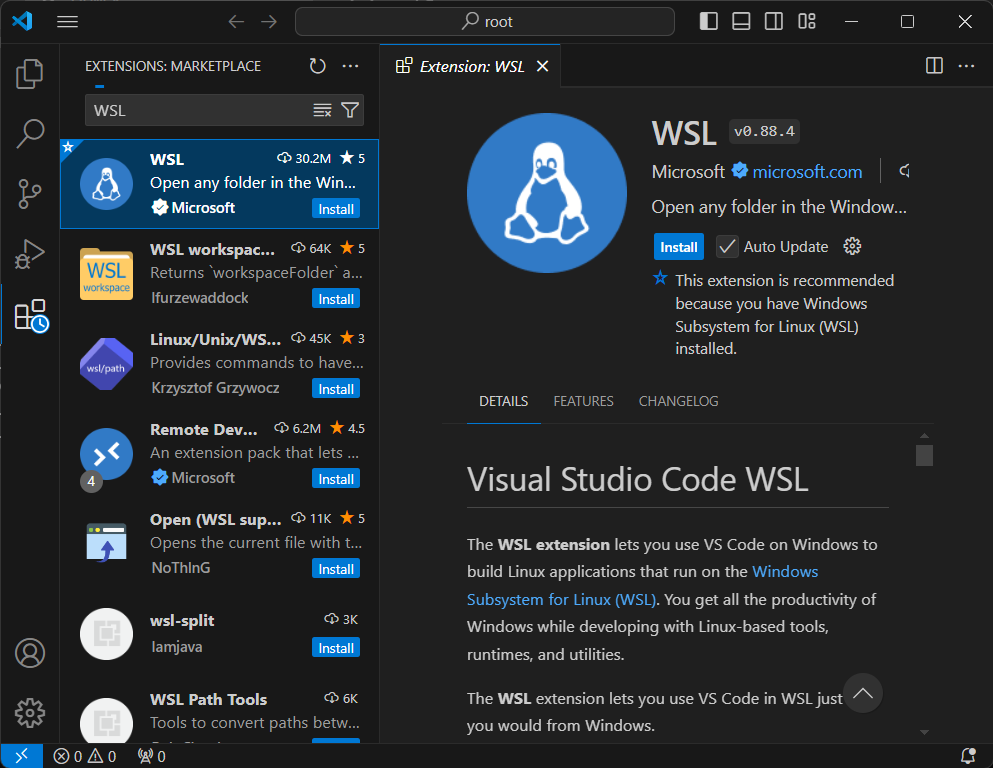
\includegraphics[width=0.8\textwidth]{Homeworks/1-Hello-World/wsl-extension.png}
\end{center}

Исчерпывающее руководство по установке WSL представлено
\href{https://learn.microsoft.com/ru-ru/windows/wsl/setup/environment}{тут}.
Установка сводится к выполнению в командной строке Windows команды:

\begin{terminalwindow}{terminalhomework}
!\shellcommand{wsl --install}!
\end{terminalwindow}

После выполнения этой команды и перезагрузки компьютера в списке установленных приложений
должно появиться приложение Ubuntu.
Для проверки совместной работы WSL и VSCode на хостовой системе можно в консоли WSL выполнить
команду:

\begin{terminalwindow}{terminalhomework}
!\shellcommand{code .}!
\end{terminalwindow}

Должен открыться редактор VSCode в директории, из которой была выполнения команда.

После этого можно установить в WSL компилятор и другие инструменты разработки:

\begin{terminalwindow}{terminalhomework}
!\shellcommand{apt update}!
!\shellcommand{apt install -y build-essential cmake}!
\end{terminalwindow}

Для проверки успешности установки инструментов разработки, предлагается выполнить команды:

\begin{terminalwindow}{terminalhomework}
!\shellcommand{g++ --version}!
!\shellcommand{make --version}!
!\shellcommand{cmake --version}!
\end{terminalwindow}

\section{Hello World!}

После установки всех необходимых программ можно приступить к написанию первого проекта.
Весь исходный код для проекта представлен в домашней работе, поэтому требуется только следовать
инструкциям.

\begin{enumerate}

        \item В рабочей директории создать директорию hello-world и перейти в нее:

            \begin{terminalwindow}{terminalhomework}
!\shellcommand{mkdir hello-world}!
!\shellcommand{cd hello-world}!
            \end{terminalwindow}

        \item Открыть VSCode в директории hello-world:

            \begin{terminalwindow}{terminalhomework}
!\shellcommand{code .}!
            \end{terminalwindow}

        \item В VSCode создать файл main.cpp со следующим содержимым:

            \myinputlisting[minted language=cpp]
                {Homeworks/1-Hello-World/}
                {main.cpp}

        \item Создать проектный файл CMakeLists.txt со следующим содержимым:

            \myinputlisting[minted language=cmake]
                {Homeworks/1-Hello-World/}
                {CMakeLists.txt}

        \item Собрать программу:

            \begin{terminalwindow}{terminalhomework}
!\shellcommand{cmake -B build}!
!\shellcommand{cmake --build build}!
            \end{terminalwindow}

        \item Выполнить собранное приложение:

            \begin{terminalwindow}{terminalhomework}
!\shellcommand{./build/main}!
            \end{terminalwindow}

\end{enumerate}

\end{document}
